% Created 2023-02-21 Di 20:37
% Intended LaTeX compiler: pdflatex
\documentclass[11pt]{article}
\usepackage[utf8]{inputenc}
\usepackage[T1]{fontenc}
\usepackage{graphicx}
\usepackage{longtable}
\usepackage{wrapfig}
\usepackage{rotating}
\usepackage[normalem]{ulem}
\usepackage{amsmath}
\usepackage{amssymb}
\usepackage{capt-of}
\usepackage{hyperref}
\usepackage[a4paper,width=160mm,top=25mm,bottom=25mm]{geometry}
\author{Geeju Kwon, Jiawei Sun, Philip Wolper}
\date{\today}
\title{Simulation of wheat yield in the Cerrado region of Southern Brazil using the SIMPLE crop model}
\hypersetup{
 pdfauthor={Geeju Kwon, Jiawei Sun, Philip Wolper},
 pdftitle={Simulation of wheat yield in the Cerrado region of Southern Brazil using the SIMPLE crop model},
 pdfkeywords={},
 pdfsubject={},
 pdfcreator={Emacs 27.1 (Org mode 9.6)}, 
 pdflang={English}}
\begin{document}

\maketitle

\section{Introduction}
\label{sec:org1419b69}
The Cerrado region of Brazil refers to the tropical savanna biomes that are widely distributed in the Eastern states of the country. In general, the climate of Cerrado region is characterized by the semi humid tropical regimes that are dominated by wet and cold seasons annually. Conventionally, Brazil’s wheat production is distributed in the Southern regions of Brazil, contributing up to 91 \% of national production in 2017. Although not considered a traditional region of cereal production, the Cerrado has become the target of agricultural expansion since the 1980s, due to its potential to grow wheat in the off-seasons from that of the Southern regions. It is worth noting that the Cerrado is a topic of interest due to its unprecedented agronomic background. For example, the seasonal variation of water usage and the blast disease caused by the fungus \emph{Pyricularia oryzae} are identified as significant threats to long-term productivity and yield stability. The incentive of agricultural expansion into the Cerrado is considered to be a lucrative development in the region, partitioning approximately 44\% of its total area to farmland. However, Brazil’s agroeconomic reliance on such expansions may highlight the increasing vulnerability to anthropogenic climate change, which could destabilize crop production to meet the domestic food demand. Recognizing the impacts of the progressing agricultural expansion, the employment of crop system simulations could offer a sustain growth model for shareholders, legislators, and farmers. Moreover, the development of simulated crop models could illuminate the crucial system components and its interrelationships involved in crop production, overcoming agronomic challenges.

\begin{figure}[htbp]
\centering
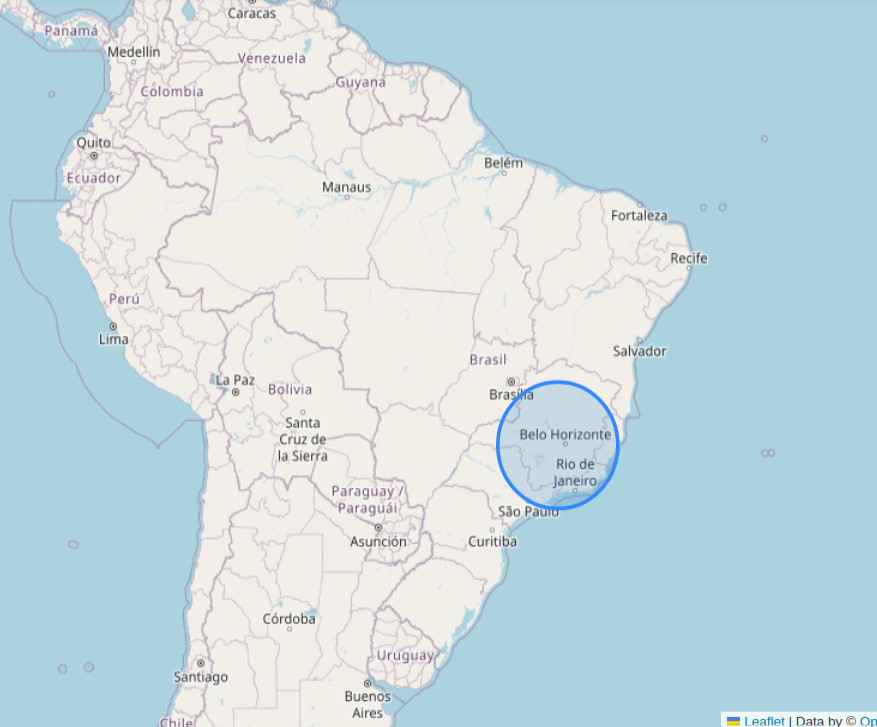
\includegraphics[width=0.5\textwidth]{./figures/Brazil with cerrado.png}
\caption{Relative location of the Cerrado in Brazil. The circle encloses the area .}
\end{figure}

\section{Objectives and Aims}
\label{sec:org2511eb1}
This study aims to utilize the SIMPLE crop model developed by Zhao et al. to simulate crop production in the Cerrado region at various locations and temporal scales. Additionally, this study intends to explore the model’s statistical fit for wheat yield simulations in relation to the observed experimental data. Simultaneously, the model’s response to a changing climate will be assessed under the conditions presented in Representative Concentration Pathways climate change model. Although several models have been extensively developed for wheat, the SIMPLE crop model is selected for the study due to its relatively simple yet dynamic nature. Notably, the integration of widely understood processes with few parameters and data requirements that exclude crop-specific processes, is considered the appeal of utilizing the SIMPLE model.

\section{Experimental Data}
\label{sec:orgaa47948}
Experimentally determined wheat yield was collected for 13 field trials from five experimental sites located in the Cerrado (Rio Paranaíba, Viçosa, São Gotardo, Sete Lagoas, and Itutinga) (\textbf{Table and Figure}, who to site). The field trials were conducted between 2018 and 2021 and were conducted with the wheat cultivar BRS264, which is the most widely grown and consumed culitvar in the Cerrado since the last 10 years, due to its tolerance to heat, pathogens, water lodging and toxic metal elements commonly found in Cerrado soils (\textbf{cited by Sun: BRS264 P5}). While the sowing date varies between locations and experiments, on average the wheat was sown on the 20th of May and harvested on the 19th of September. This timeline coincides with the recommendation for this cultivar (\textbf{cite by Sun: ''BRS264 P9 and P11''}). Because we did not have access to detailed soil data for each location, soil parameters were approximated from the average content of clay, sand and silt in the Cerrado (\textbf{site soil content}). Using the Unified Soil Classification System Pyramid, this yielded a soil with sandy loamy characteristics. The 13 field trials included both irrigated and non-irrigated experiments, but no further data on the amount of irrigation was supplied. While for most field trials various environmental conditions are controlled such as nutrient saturation and disease control, it is very important to note that wheat grwon under nonirrigated conditions in the location São Gotardo was artificially inoculated with the fungal pathogen \emph{Magnaporthae oryzae} pv. \emph{Triticum}, which causes wheat blast disease (cited by Sun 'BRS 264 P10').

\begin{figure}[htbp]
\centering
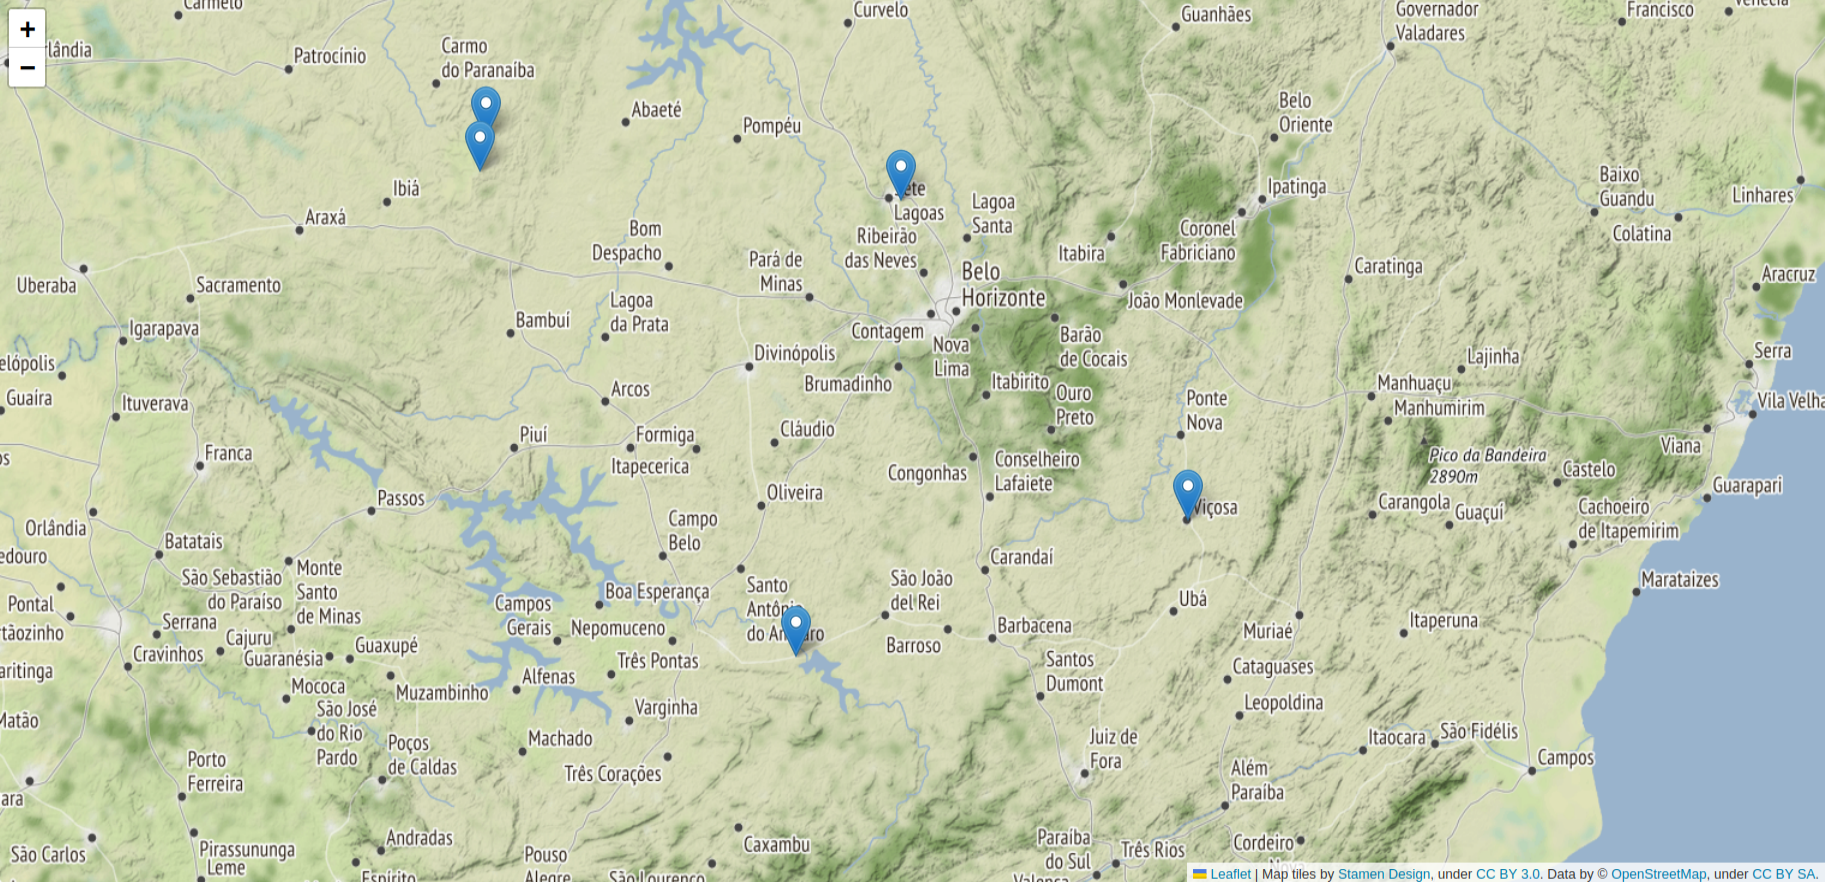
\includegraphics[width=1\textwidth]{./figures/Brazil.png}
\caption{Location of the field trials in the Cerrado in Brazil, which were simulated in this study.}
\end{figure}

\begin{table}[htbp]
\caption{\label{list}List of 13 field trials used in this study, adapted from Casagrande, 2023. (*field trials inoculated with blast)}
\centering
\begin{tabular}{|ccccc|}
\hline
Year & Location & Water & Name & Trial period\\
\hline
\hline
2018 & Rio Paranaiba & no & irrigated & May-September\\
\hline
2019 & Rio Paraneiba & no & irrigated & May-September\\
\hline
2019 & Vicosa & no & irrigated & June-October\\
\hline
2020 & Vicosa & no & irrigated & June-October\\
\hline
2020 & Vicosa & yes & nonirrigated & June-October\\
\hline
2021 & Vicosa & no & irrigated & June-October\\
\hline
2020 & Sao Gotardo & no & irrigated & May-August\\
\hline
2020 & Sao Gotardo* & yes & nonirrigated & July-November\\
\hline
2021 & Sao Gotardo & no & irrigated & April-September\\
\hline
2021 & Sao Gotardo* & yes & nonirrigated & March-August\\
\hline
2022 & Sao Gotardo* & yes & nonirrigated & March-August\\
\hline
2020 & Sete Lagoas & no & irrigated & July-November\\
\hline
2021 & Itutinga & yes & nonirrigated & March-August\\
\hline
\end{tabular}
\end{table}

\section{SIMPLE model}
\label{sec:org5b61a63}
The SIMPLE crop model was used as outlined by Zhao et al., modelling our desired crop growth, development, and yield using a daily time step. In general, the input parameters of this experiments were adapted to account for the effect of daily temperature, heat stress, rainfall, and atmospheric CO2 concentration. Several assumptions were taken into consideration to effectively simulate the biological systems involved. 
For example, with the aim to keep the model simple to utilize, the accumulation of phenological temperature for maturity began when it was above the base temperature for the crop series. This process did not account for an optimum temperature threshold, and omitted any other growth stages. Additionally, the model acknowledged that photosynthesis is a function of radiation use efficiency, with biomass growth converted from the daily active radiation intercepted by the canopy. Based on this, the biomass accumulation was calculated as a product of radiation, fraction of intercepted solar radiation, radiation use efficiency, fraction of temperature and atmospheric carbon dioxide. Similarly, the final yield of wheat from the Cerrado region was calculated as the product of accumulated biomass and its specific harvest index. It is worth noting that to account for heat stress, the SIMPLE model considers the fraction of water, temperature, and heat, but disregarded leaf area index.
As emphasized earlier, the SIMPLE model integrates widely understood processes by simplifying data requirements outside of crop-specific processes. Hence, the simulation of Cerrado grown wheats utilized the sowing/harvesting date, irrigation status, and the initial variables as provided by the experimental data. Additionally, the weather inputs that pertain to temperature, rainfall, and fraction of solar radiation were adapted from measurement data from NASA POWER. During initialization, any specific parameters such as species parameters, not provided directly by the SIMPLE model, were set manually to calibrate the model. 
The calibration process involved executing the model to observe whether it was able to simulate the cultivar parameters at different locations and time frames within reasonable ranges. As such, throughout the calibration process, several parameters were adapted from the weather data. For instance, the concept of I50A and I50B were introduced to express the cumulative temperature required for leaf area development to intercept 50\% of solar radiation during canopy closure, and cumulative temperature required from maturity to 50\% of radiation interception during canopy senescence, respectively. For the cultivar parameters for BRS264 used in this study, the calibration process involved the adjustment of the I50A and I50B values to 500 and 300 from the dataset provided. Simultaneously, the harvest index of the strain was set to 0.34 to best reflect the growth conditions it was exposed to. 
Furthermore, to calibrate the model, specific irrigation treatments of the experimental locations was considered. This is due to the experimental data exposing the same cultivar to alternating irrigation conditions in different years and locations. Based on literature, these different irrigation treatments were identified as experiments that tested for the best strategies of cultivation in the Cerrado during the off-seasons of wheat cultivation under water-stressed conditions. As such, the model simulated all the experimental datasets under the assumption of irrigation conditions. This was justified as the scope of this investigation does not simulate the yield under water-stressed conditions. Moreover, this assumption would allow the study to avoid skewing the model’s yield simulation due to lack ability to distinguish each condition of the experimental location, which could ultimately influence the sensitivity of the model. Lastly, as the SIMPLE model does not account for nutrient dynamics, this study did not accept potential nutrient treatments as an input parameter.


\section{Results}
\label{sec:org33b62c0}
\subsection{Simulated experiments}
\label{sec:org1ebcbc5}
In order to assess the capabilities of the SIMPLE model to model wheat growth in the Cerrado region, we simulated yield for 13 field trials in 5 different locations. Irrigated location where simulated with no water stress, implying a perfect watering routine. Nonirrigated crops had water stress turned on and relied only on rainfalls, supplied in the weather data. Since no nutrients are simulated in the SIMPLE model, we assume perfect nutrient saturation of the crops, a state not uncommon for field trials. The atmospheric CO2 concentration was set to 415 ppm, reflecting the current value as of 2020. Soil parameters were estimated from the content of Silt, Clay and Sand found in typical Cerrado soils (\textbf{cite soils})
The species and cultivar parameters required by the SIMPLE mode were derived from literature or estimated based on similar species. (\textbf{cite zhao et al.}) Further calibration was done by adjusting cultivar parameters (Tsum, I50A, I50B and HI) within reasonable levels.
The results of the simulation across experiments are shown in (Figure calibration). The model has an relative root mean square error across all trials of 39.1\%:

\begin{figure}[htbp]
\centering
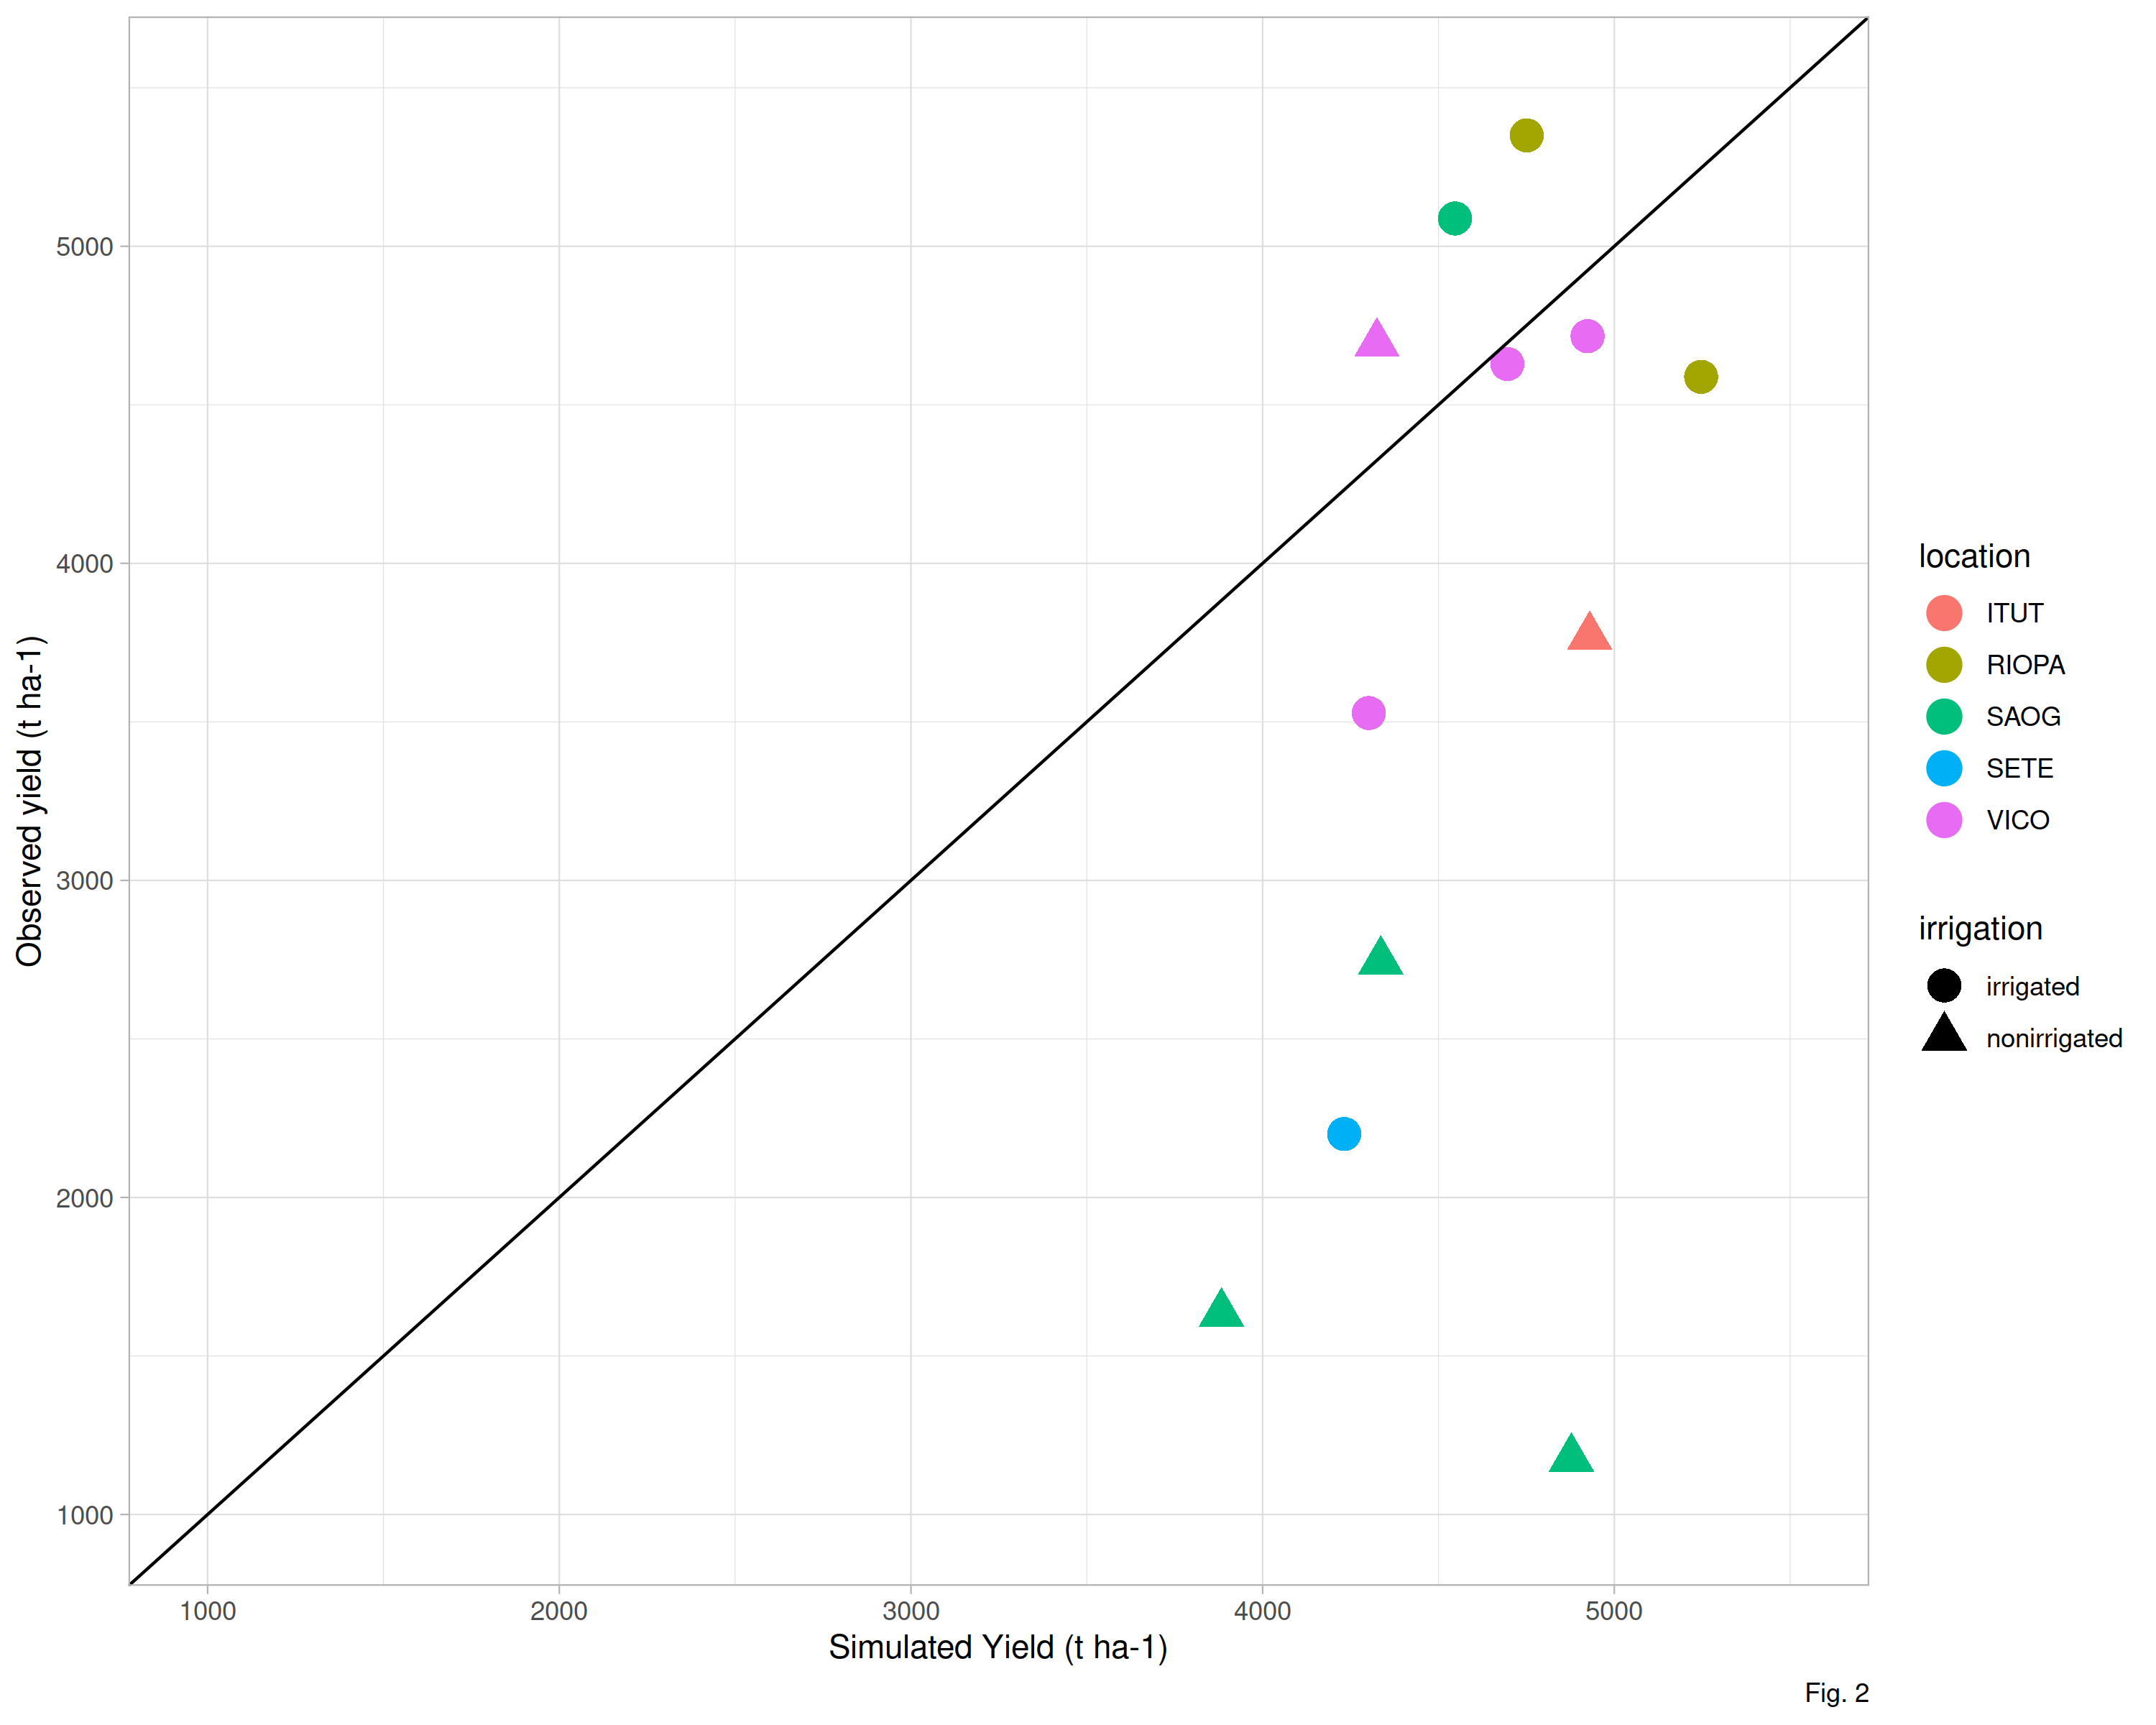
\includegraphics[width=0.8\textwidth]{../results/experimental-data/2023-02-18_Obs_Sim_all_415.png}
\caption{\label{obs-sim}Simulated vs. Observed yield for 13 field trial locations in the Cerrado, Brazil.}
\end{figure}

These results indicate that in many cases there is significant deviation between the simulated and observed yield. While several experiments are simulated with decent accuracy, a general trend of the simulation to overestimating the observed yield can be observed. Due to the simple nature of the model this is to be expected, since in reality there are many more yield-limiting factors, such as nutrients, that the SIMPLE model does not account for.
We also observe that the accuracy of predicting yield varies significantly between locations, as can be expected between differing environments. Experiments conducted in Vicosa, MG are the most accurately simulated of all 5 locations with a RRMSE of 10.1\% (see Figure \ref{Vicosa}).
On the other hand, specifically the nonirrigated field trials in Sao Gotardo, which  have been inoculated with a fungal pathogen, show a bad fit between simulated and observed yield, grossly overestimating the yield in the simulation. This discrepancy is likely caused by the fungal pathogen having a negative effect on the yield, which is not accounted for by the model. When excluding these locations from the simulation, the accuracy of our model improves to 20.1\%.

\begin{table}[htbp]
\caption{\label{stats}Model statistics}
\centering
\begin{tabular}{|c|c|c|c|c|}
\hline
 & r\_squared & mae & rmse & md & rrmse\\
\hline
All & 0.226 & 1131.89 & 1499.29 & 0.435 & 39.1\%\\
healthy & 0.254 & 717.22 & 890.4 & 0.349 & 20.1\%\\
Vicosa & 0.336 & 354.35 & 442.34 & 0.479 & 10.1\%\\
\hline
\end{tabular}
\end{table}

Summary statistics decribing the accuracy are done for all experiments, as well as subgroups of the data. These can be seen in Table \ref{stats} and include all the experiments (All), excluding the nonirrigated trials in Sao Gotardo, where the plants were infected with the blast fungus (healthy) and statistics of only the trials in Vicosa (Vicosa), where the model performed the most accurately (see Fig \ref{Vicosa}).

\begin{figure}[htbp]
\centering
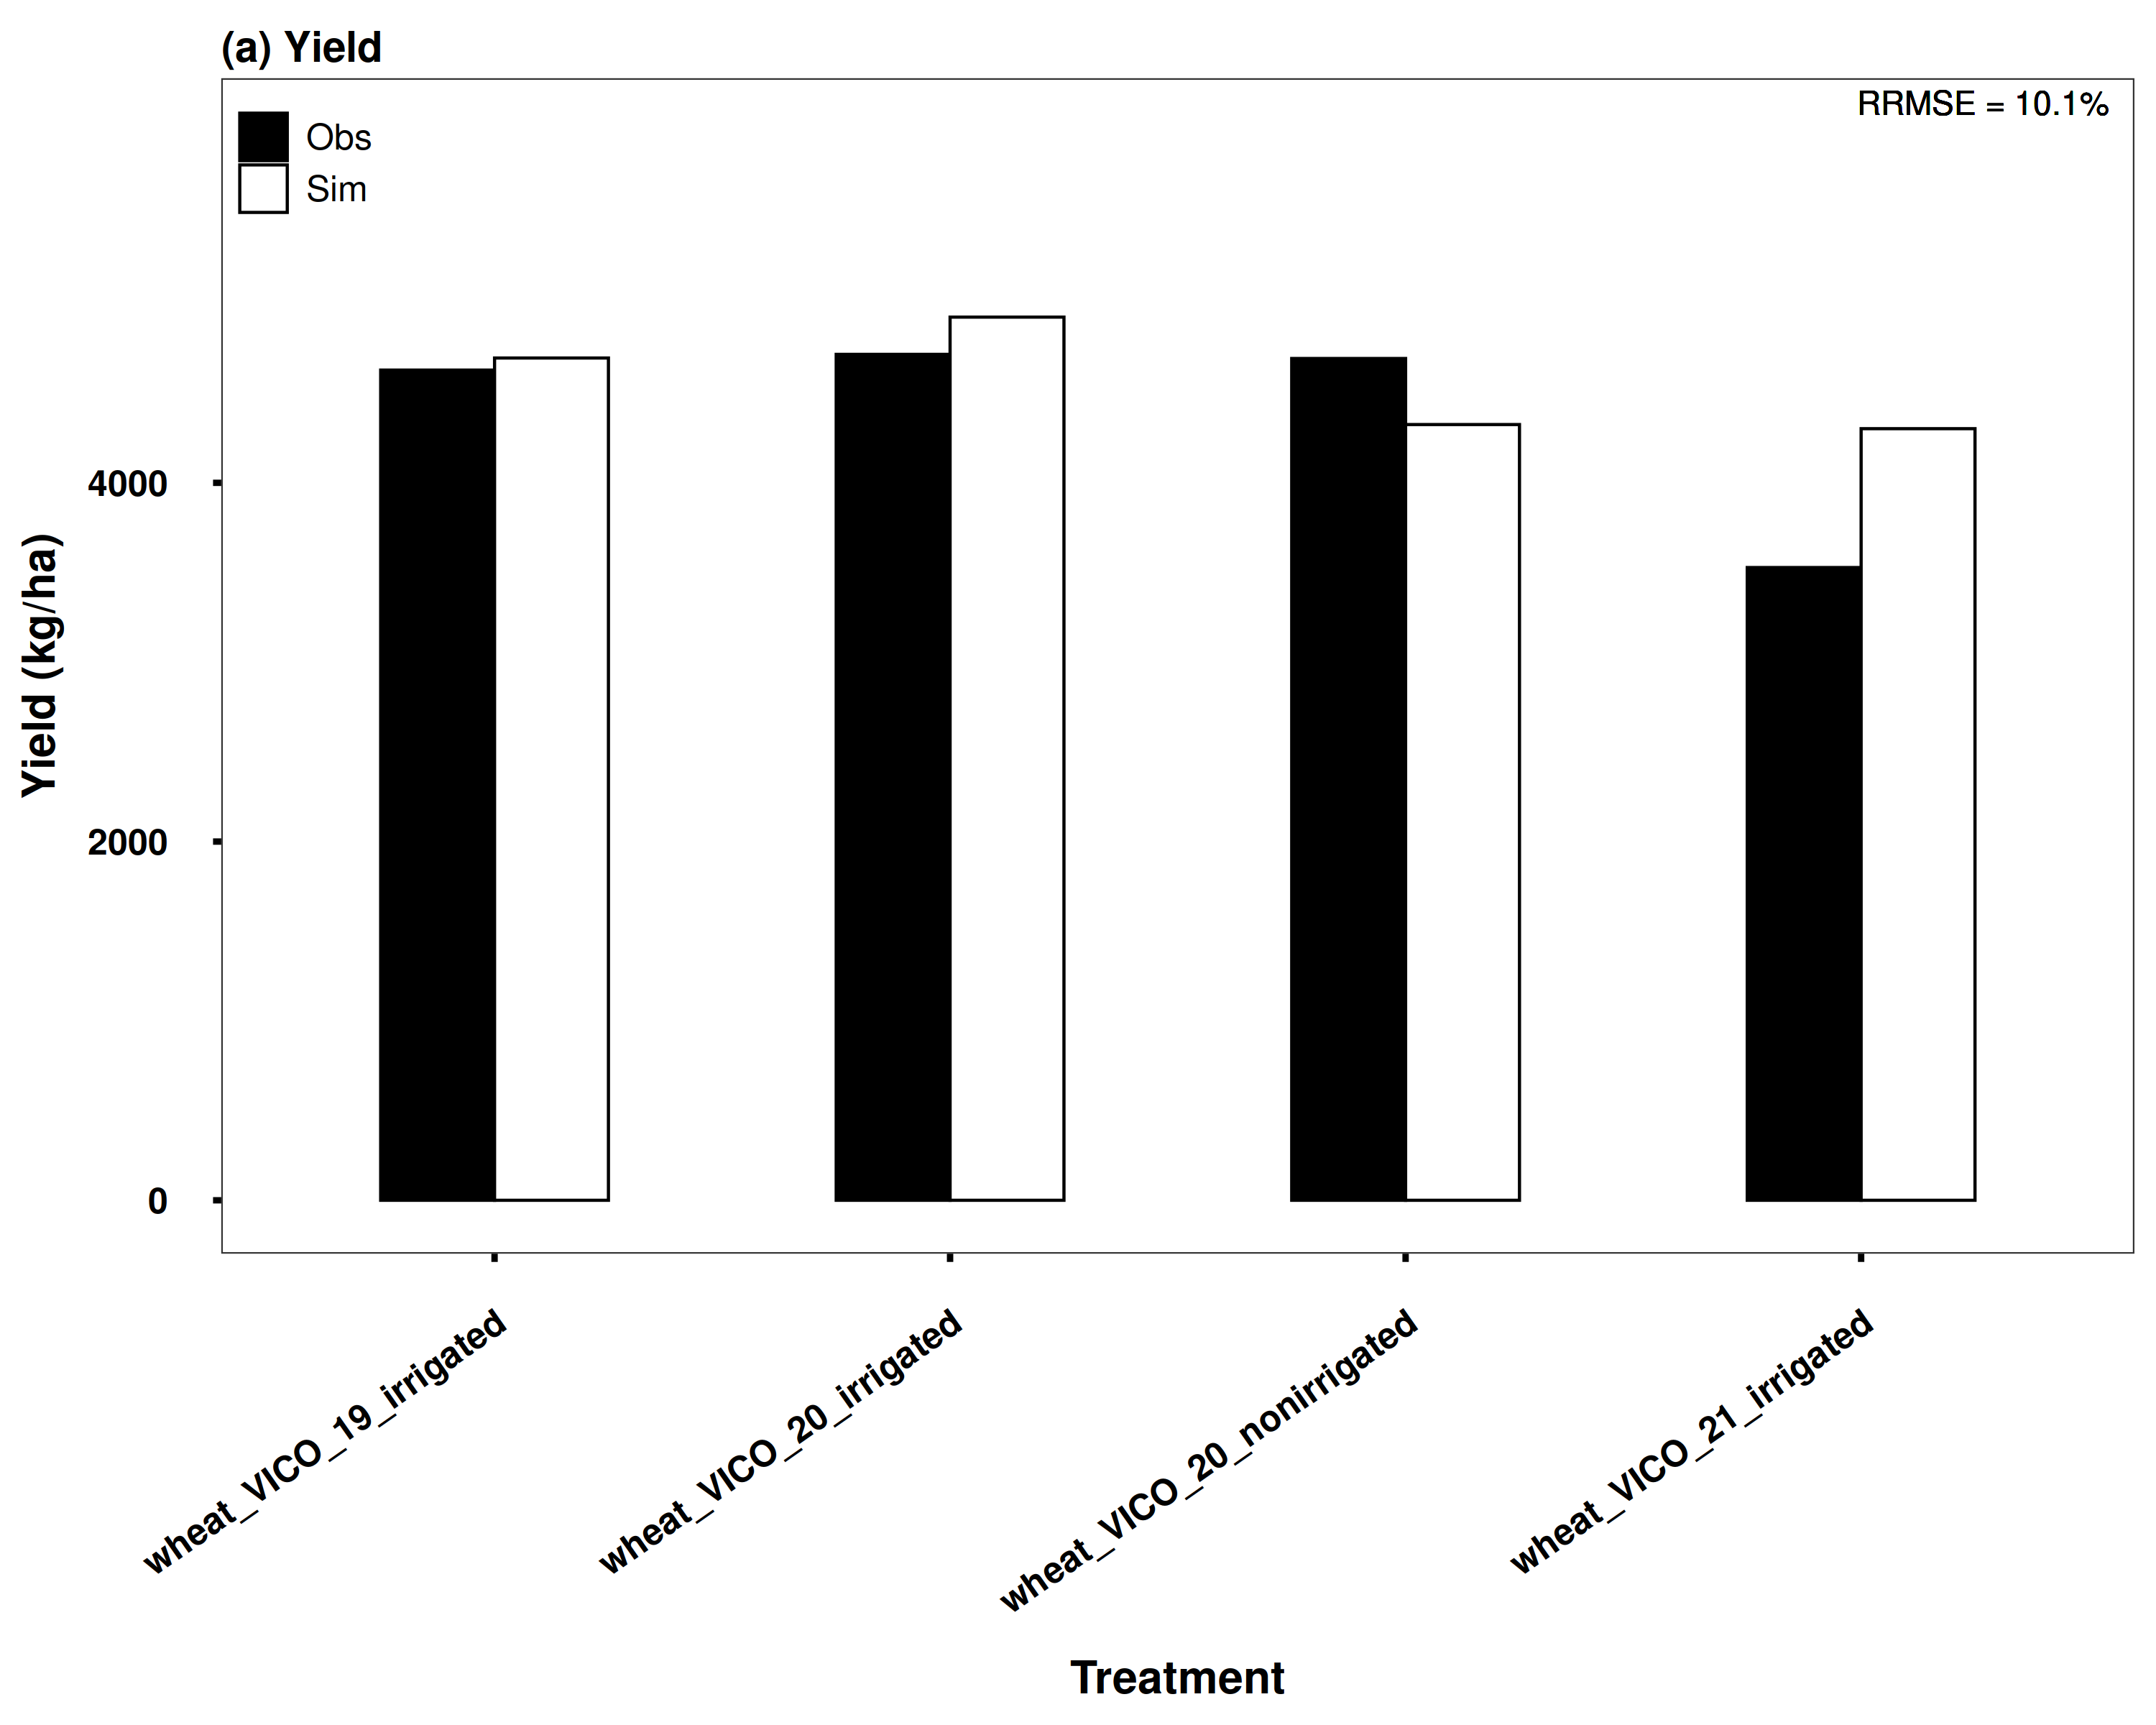
\includegraphics[width=0.8\textwidth]{../results/experimental-data/2023-02-18_Vico_only.png}
\caption{\label{Vicosa}Simulated yield for four field trials located in Vicosa, MG, Brazil.}
\end{figure}


\subsection{Climate change prediction}
\label{sec:org687eaff}
In order to predict the effect climate change can have on wheat cultivation in the Cerrado, we simulated 70 years of wheat yields from the year 2030 until 2099. The simulations were conducted using the same parameters as the calibrated SIMPLE model. Environmental conditions such as temperature, rainfall and irrigation were obtained from a climate prediction model, which supplied daily weather data for the from 2030 until the end of the century. The location predicted by the climate model is Brasilia, Brazil, the country's capital located approximately 600 km northwest of the location of our trials, but still in the Cerrado.

To assess the effects of the predicted climate on crop growth we conducted simulations first keeping the atmoshperic CO\textsubscript{2} concentration constant at 450 ppm, a value slightly higher than currently and realistic for 2030 (see Figure \ref{cc-model}A). Under theses conditions the wheat yield shows a visible decline, decreasing from around 4000 t ha\textsuperscript{-1} in 2030 to approximately 2600 t ha\textsuperscript{-1}. Additionally the varies strongly from year to year, and there is almost no stable yield over multiple years. In some cases the yield is reduced by as much as 60\% compared to the previous year, as seen 2093-2094. Although cases of extremely low or higher than average yields are very common in our simulations, we do not find the occurence of these extreme event to significanlty increase in frequency as the years progress. Nevertheless, we simulate a significant decline in yields over the century, with constant CO\textsubscript{2}.

As the amount of greenhouse gases (GHG) released by humans and their societies predicted to further increase during the second half of the century it, it is important to understand the impact of increased GHGs on agriculture. As it is the most common GHG emitted by humans and contributes greatly to global warming the levels of CO\textsubscript{2} in the atmosphere have been subject to much predictive modeling. According to the latest IPCC (\textbf{cite}) report, by the end of the 21st Century the concentration of CO\textsubscript{2} in the atmosphere is predicted to increase to levels anywhere between 400 ppm to 1100 ppm. While the lower limit of this prediction depends on the most favorable scietal drivers involving drastic reductions in emission very rapidly, the upper limits assumes the most detrimental course of society, involving little to no climate action. While both of these szenarios are considered unlikely, mean CO\textsubscript{2}-concentration in the atmosphere is still likely to increase by up to 50\% under realistic szenarios.

In order to simulate the effect of increasing atmospheric CO\textsubscript{2} concentrations on wheat yield in the brazilian Cerrado, we will assume a linear increase of CO\textsubscript{2} and reaches 795 ppm by the year 2100. Because our simulation starts in the year 2030, we have choose an appropriate concentration of 450 ppm as a starting value, and assume an increase by 5 ppm. The weather data is the same as for the simulation with constant CO\textsubscript{2} levels.
In contrast to the unchanging CO\textsubscript{2} concentrations, the increase in CO\textsubscript{2} does not lead to an immediate decline in yield. Interestingly, for approximately the first half of the simulated timeframe we see a slight increase in the yield. After increasing by about 500 t ha\textsuperscript{-1}, after the year 2075 the yield starts to drop again ending with values similiar to 2030.

\begin{figure}[htbp]
\centering
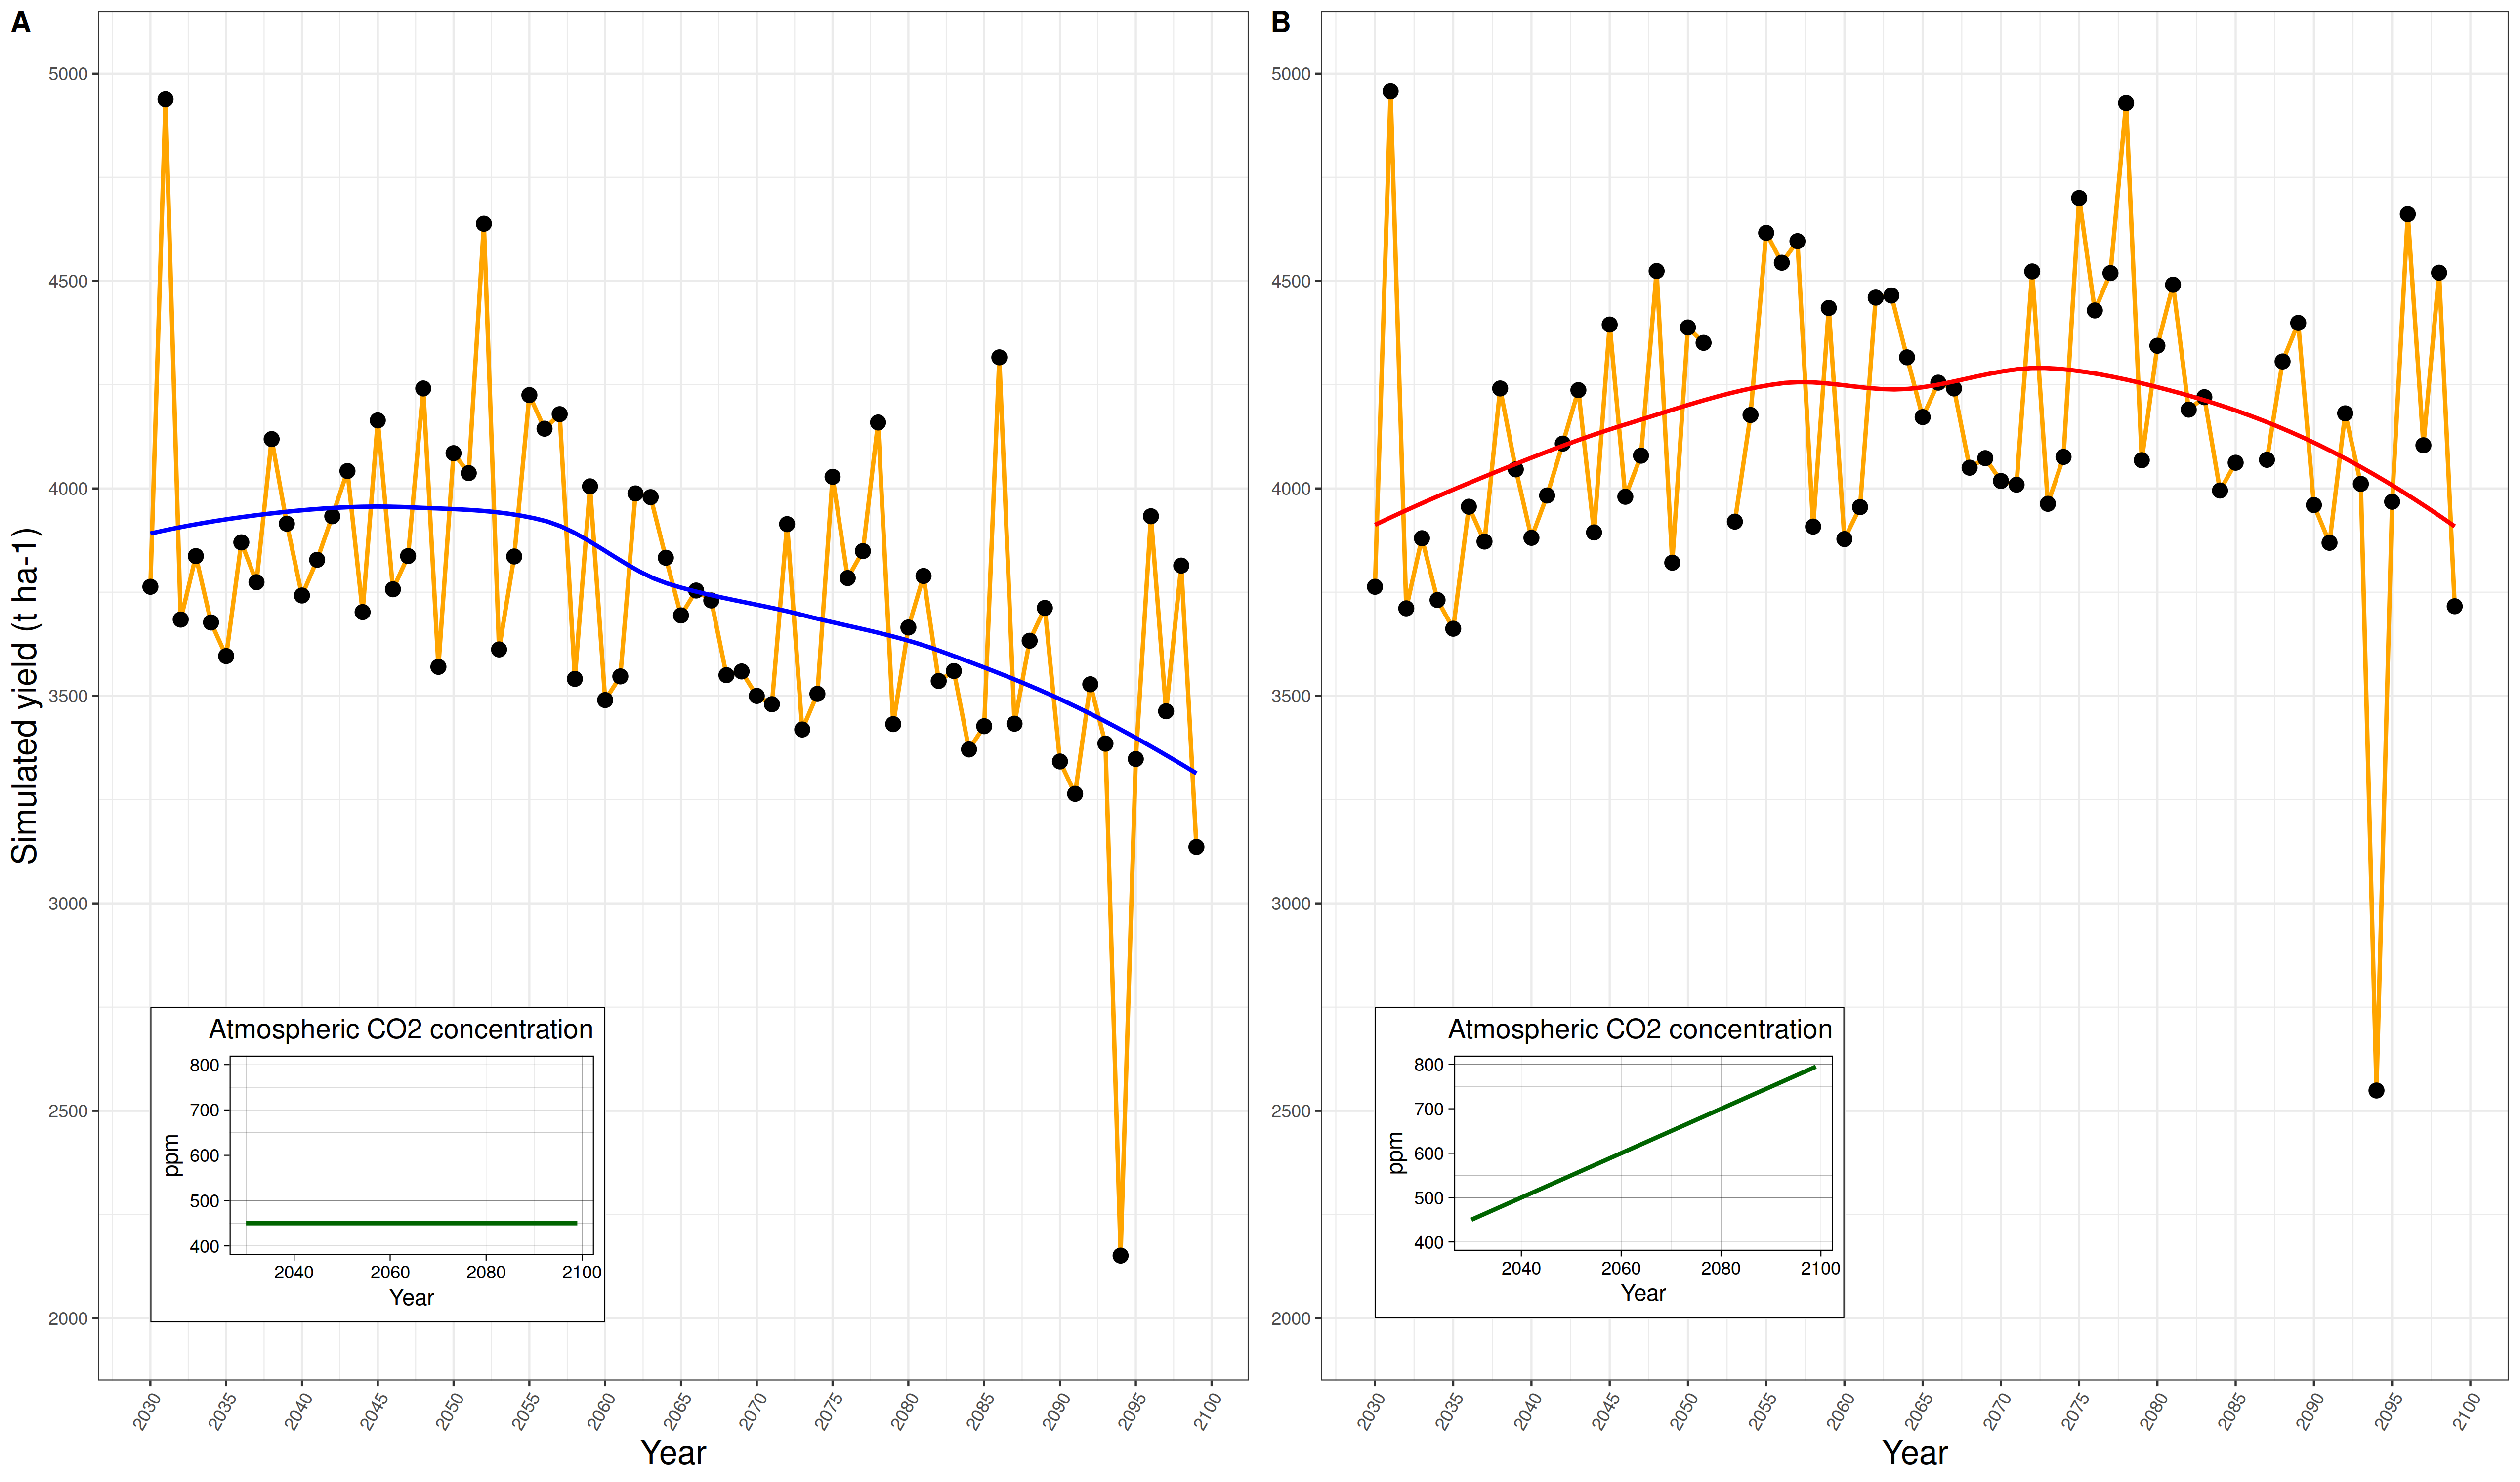
\includegraphics[width=1\textwidth]{../results/cc-model/2023-02-21_yield_prediction_cc_model_CO2_with_conc.png}
\caption{\label{cc-model}Climate change model}
\end{figure}


\subsection{Decreasing yield is due to higher temperature accelerating senescence}
\label{sec:orga250ee3}
To understand the underlying factors contributing to the similated decreasing yield in the Cerrado, it is necessary to identify possible causes and how the SIMPLE model implements these. While a decrease in yield is often associated with different types of crop stress, we aim quantify the stresses contributing to the decreasing yield in our simulation. While an increasing average daily maximum temperature (Fig. \ref{paras-sim}A), could indicate heat stress, the factor responsible for heat stress, F\_heat, remains relatively constant and only shows slight heat stress in the mid 2090s (Fig. \ref{paras-sim}B). An alternative cause could be water stress, which could be an indirect effect of high temperature. But when observing the simulated factor responsible for water stress F\_Water (Figure \ref{paras-sim}C), this too remains constant over the course of the simulated time frame.

\begin{figure}[htbp]
\centering
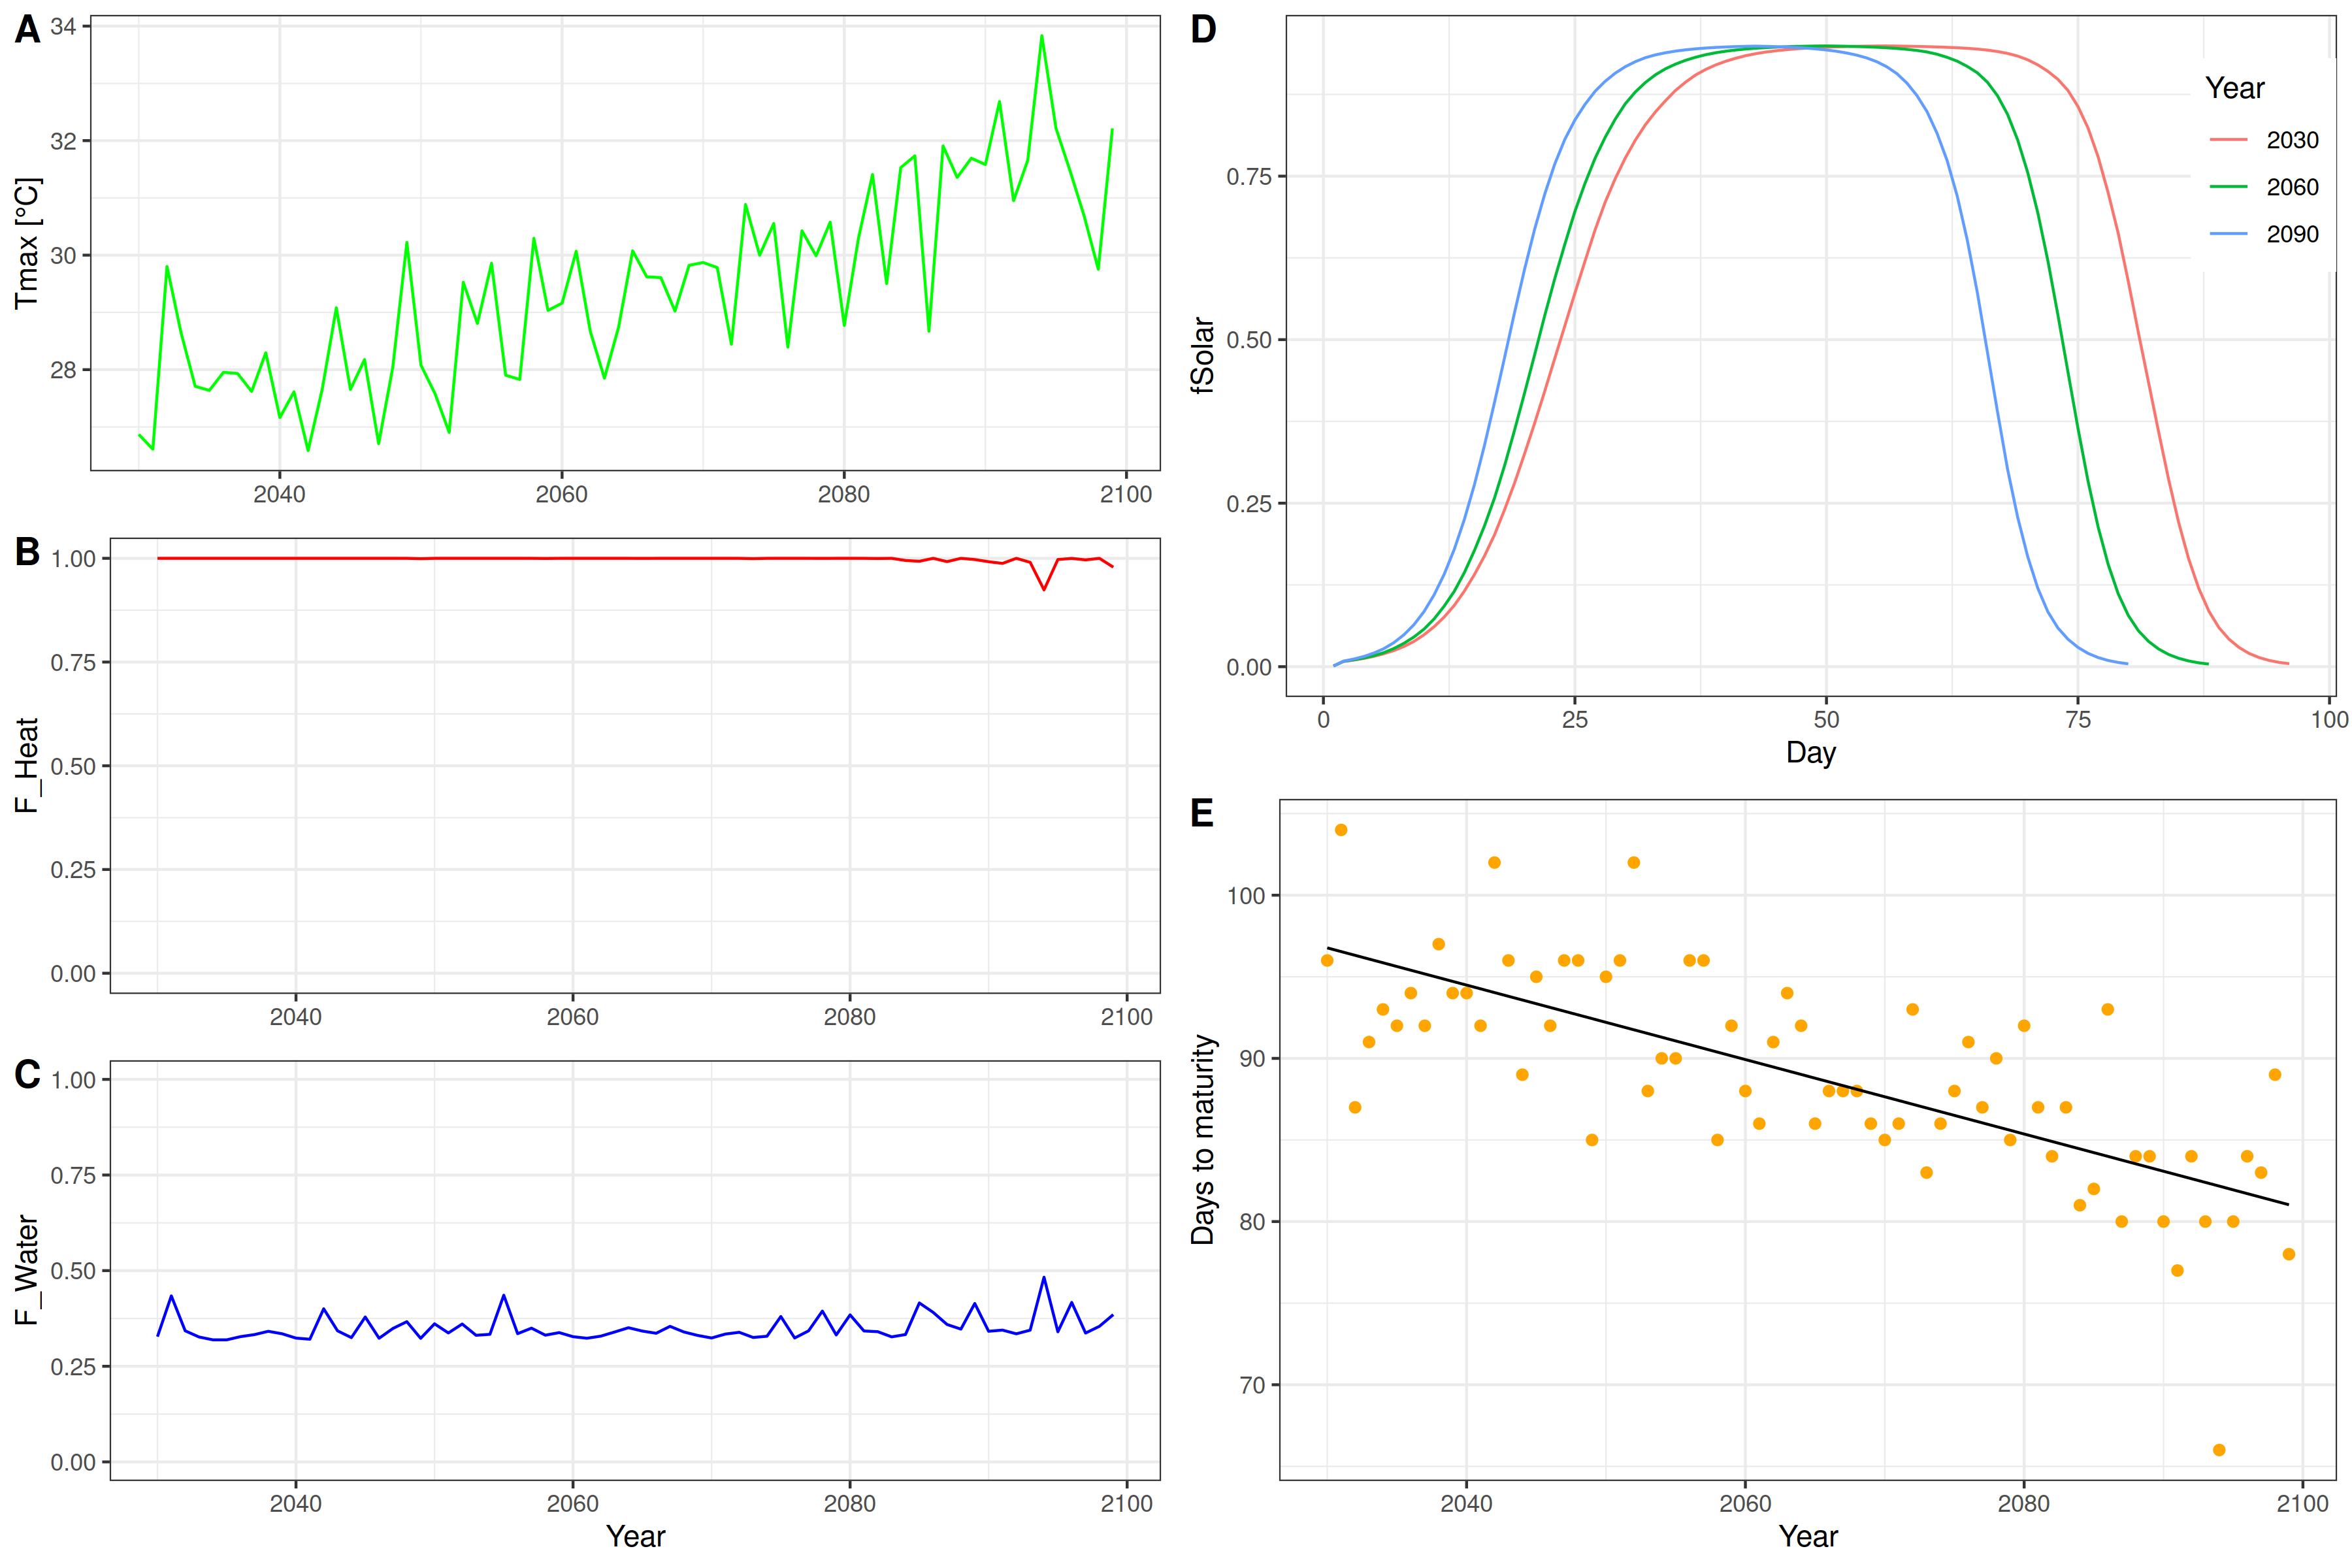
\includegraphics[width=1\textwidth]{../results/cc-model/paras_sim.png}
\caption{\label{paras-sim}Crop simulation parameters for simulation with constant CO\_2 concentration.}
\end{figure}

When observing the change in the fraction of solar radiation, fSolar, intercepted by the plant at a given point in its development, we can se that the plant reaches maturity, before decreasing again after the plant reaches maturity.
When comparing the fSolar curves between simulated years (Fig. \ref{paras-sim}D), we can see that the crop reaches full photosynthetic capabilities earlier and earlier for simulations closer to the end of the century. Additionally, the days it takes for the crop to reach maturity also decrease, indicating that the plant also starts senescence earlier, loosing biomass again. When combined with the constant harvest date of 110 days after sowing used in this simulation, this explains the reduction in yield. Since the phenology and therefore the maturity is contolled by the temperature, a yearly increase in temperature will affect the simulation by reducing yield.


\section{Discussion}
\label{sec:orgb297d08}
While the SIMPLE model, lacks much of the complexity of other crop models it is remarkable, that we were able to simulate wheat fairly accurately. Our SIMPLE model had an RRSME of 20.1\%, when excluding field trials infected with blast, which is comparable to the RRMSE of 11-24\% using multiple wheat models in a study done by \textbf{Asseng, 2015, cite}. While we acknowledge, that our data set was likely more homogenous than other studies, it still shows the capabilities of the SIMPLE model to accurately simulate crop growth if supplied with appropriate input variable and high quality datasets.

As with many crop models, the simulated yield is more a representation of the attainable yield under limiting factors such as water, than the actual yield. The later is additionally influenced by reducing factors such as diseases, weeds or pollutants. These reducing factors are not in the scope of the SIMPLE model and many times are a reason for the discrepancy between simulated and observed yields. Important to note are the cases in which a parameter influences the behavior of the model more strongly than is the case in the actual production situation, leading to a higher observed yield than simulated. Indentifying such cases requires good understanding of the model as well as the biology of the crop.

An important drawback of the SIMPLE model is that it does not account for nutrient-dynamics. In case of the field trials we have assumed, that crops would be optimally managed and thus not lack any major nutrients. This might not be the case in all production-situations across the globe, especially in areas lacking technological farming equipment and resources such as sub-saharan Africa or southeast Asia. When trying to apply the model to such locations it is important to acknowledge the limits this might impose on its accuracy. On the other hand the SIMPLE model is very well suited to being applied to novel locations and less studied crops, due to its limited amount of required input parameters. Adding additional modules, to simulate nutrient-dynamics for example, could improve the usage of the SIMPLE crop model as an easy to implement crop model around the world.

One goal of this study was to assess the agricultral potential of the Cerrado region in Brazil in the light of changing environmental conditions in the second half of this century. We were able to simulate yield for 70 years based on weather data of a climate model, under two different atmoshperic CO\textsubscript{2} scenarios, increasing and constant. Both scenarios revealed a decrease on yield in the fourth quarter of the century due to increased temperature. These results are somewhat consistent with predictions of agricultural development in the light climate change generally, with global warming and depletion of groundwater resources causing more long periods of heat stress and drought in crop systems on average (\textbf{citation}).

A vital point here is that although the results of our simulation seem to agree with this widely accepted fact, the cause for yield decline are not due to heat or water stress as we have shown. Instead the SIMPLE model assumed heat-driven phenological development, causing faster maturation and together with the fixed harvest date used in our simulation lead to greater senescence and thus declined yield. Under real production, this would not happen because the farmer would likely harvest his field earlier. Interestingly, we observed an increase in yield with increased CO\textsubscript{2} concentrations, since CO\textsubscript{2} stimulates plant growth. While this happens for the first half of the simulation the yield resturns back to starting levels, because at a concentration of 700 ppm the SIMPLE model assumes the crop is saturated. Physiologically this can be explained by closing of the stomata at high CO\textsubscript{2} concentrations. After this poin,t at around year 2075, the previously explained temperature-driven reduction of yield becomes more dominant. While the stimulation of plant growth and yield has been experimentally shown, it is unclear  how strong the effect of increasing CO\textsubscript{2} will be in terms of climate change. It is unlikely that the increased grwoth will be able to offset detrimental environmental effects such as heat stress and drought entirely.

Knowing which effects are artefacts of the model design and accounting for additional effects not simulated in the model, becomes increasingly difficult, when both end in the same result, for example decreased yield.\\

(\textbf{Transition back to Cerrdo aim})
What factors are then likely to influence the agricultural productivity in the Cerrado?

Overall, the Cerrado is a topic of interest for agronomical studies as it is a significant ecological hotspot and a frontier for Brazil’s self-sufficiency in wheat production. As development in the Cerrado regions continue, the utilization of simulated models could provide an outlook on the sustainability of agroeconomic ventures.  For example, sustainability reviews such Lahsen et al. may argue that Brazil’s cotemporary approach of emphasizing the agricultural sector’s contribution to the GDP underlies an extractivist model of development in the Cerrado. In other words, it is suggested that the role of developing such models should not be to only diagnose the bio-geophysical interactions that occurs. On a more positive outlook, the employment of simulated models could perhaps critically illuminate development pathways that contributes to furthering human well-being and environmental sustainability. Nonetheless, as this study may have demonstrated, the SIMPLE model may be best applicable when there are known principles of crop physiological parameters to manipulate, while also acknowledging the room for improvement to describe more complex interactions.

(Not sure where the following parts should go)
Although there seems to be no significant increase of extreme yields as we get closer to the end of the century, this requires more accurate climate models and simulations to say for certain.

Additionally water stress caused by depletion of groundwater reserves is likely to be an important factor as the
\end{document}
